Machine learning (ML) has become wildly popular among scientists, engineers, and even in the mainstream media, due to the unprecedented results it repeatedly provides in a multitude of areas. To name a few, we now have self-driving cars \cite{Fridman2019}; computers that can beat the best human players at complex games like StarCraft \cite{Vinyals2017}; messaging apps can that understand what you're saying \cite{Abdulkader2016, NIPS2015_5782}; many advances in computer vision such as automatic captioning \cite{Karpathy2017}; automatic fraud detection in finance \cite{DalPozzolo2015}; and automatic lesion detection in the fight against cancer \cite{Zlocha2019}.

Artificial Neural Networks (ANNs), or Deep Learning, is the key technique behind many of these advances. They are a form of supervised statistical model. That is, given a set of \(\{x \in \R^n, \ y \in \R^m\}\) labelled data points (e.g. the pixels of an image and the classification of the image), they try to learn the underlying function from input \(x\) to output \(y\). ANNs use a particular kind of function representation made from the composition of elementary functions, or neurons, and try to incrementally optimise the parameters of the neurons by comparing the output of the network against the training data. The optimisation technique applied is almost always some variant of gradient descent, and the algorithm for applying it to an ANN is known as \textit{backpropagation}. An example neural network is given in Figure \ref{fig:1-example-net}.

\begin{figure}[h!]
    \centering
    \hspace{0.5cm}
    \begin{subfigure}[]{0.4\textwidth}
        \centering
        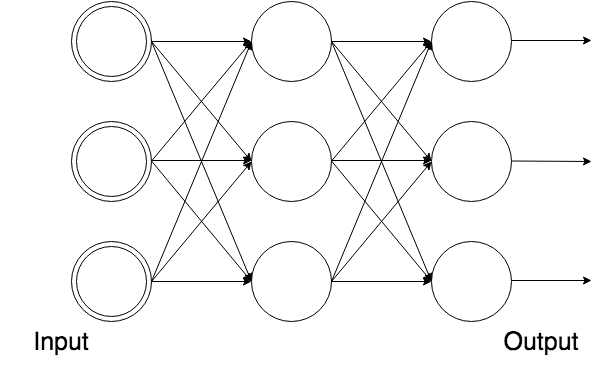
\includegraphics[width=\linewidth]{example_nn_neurons.png}
        \caption{At the individual neuron level.}
    \end{subfigure}
    \hfill
    \begin{subfigure}[]{0.4\textwidth}
        \centering
        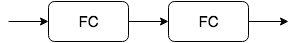
\includegraphics[width=\linewidth]{example_nn_layers.png}
        \caption{At the layer-wise level (FC means `fully connected').}
    \end{subfigure}%
    \hspace{0.5cm}
    \caption{Example ANN. The double circles denote variables rather than functions. This network would be described as a feedforward/sequential/linear network of two fully-connected/dense layers. This is because there are two layers of neurons in sequence, with each layer feeding the outputs of the previous layer to all of its neurons.}
    \label{fig:1-example-net}
\end{figure}

Training a neural network has a large memory requirement. To see how this arises, we can examine the computational (or data-flow) graph of backpropagation, as given in Figure \ref{fig:1-backprop-peak-mem}. Backpropagation has two steps, (i) \textit{the forward pass}: compute the outputs at each layer given the input, and (ii) \textit{the backward pass}: compute the gradients of the parameters at each layer given the targets and the outputs from the forward pass. As a result, the forward tensors cannot be computed in-place and must instead be kept around in memory for when the backward pass requires them. Specifically, only once \(b_i\) has been computed can \(f_i\) and \(b_{i+1}\) be freed. Therefore, as shown in Figure \ref{fig:1-backprop-peak-mem}, peak memory will occur when all the forward tensors are in memory and the first backward tensor is being computed; a linear space complexity with respect to the number of layers.

\begin{figure}[t]
    \centering
    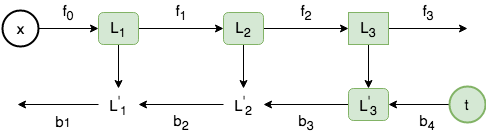
\includegraphics[width=0.85\linewidth]{backprop_overview_peak_mem.png}
    \caption{Demonstrating when peak memory occurs for the computational graph of backpropagation on a three-layer feedforward neural network. Layers in green have their output allocated in memory.}
    \label{fig:1-backprop-peak-mem}
\end{figure}

This is not good enough for large networks - as most of the layers are performing operations like multiplication on large tensors, Deep Learning can be massively sped up by exploiting the parallelism of GPUs \cite{Kayid2018, Scanzio2010, Dogaru2017}; however, state-of-the-art models have far surpassed the memory available on even top-tier GPUs and continue to get larger [?]. \todo{examples}.

This forces researchers to employ highly cumbersome and highly expensive alternatives, such as distributing the workload or developing custom hardware accelerators \todo{needs refs?}. Ideally, as the networks of tomorrow grow unabatedly, researchers should be able to focus on their experiments, rather than the complex systems problems this causes. Thus, finding a solution that can be readily implemented in existing ML software and that is transparent to the user is highly desirable, as well as orthogonal to the other approaches (which have other benefits too).

To this end, much has been done, but every memory optimisation proposed has its pitfalls. For example, quantization decreases the model's accuracy \cite{Zhou2016}; and GPU-CPU data swapping may require expert human intervention, is difficult to tractably solve for the optimal swapping strategy, and is hard to implement as you must delve deep into the ML framework's memory manager and have it precisely pipeline data transfer and computation \cite{Rhu2016, B, Zhang2019, Wang2018}.

In this thesis, I focus on a technique known as checkpointing \cite{Dauvergne2006, Martens2012, Siskind2018, Chen2016, Gruslys2016, Wang2018}, which results in large memory savings, is much simpler to implement, does not affect model accuracy and requires minimal effort from the user; though it is hard to solve tractably and, compared to a theoretically optimal swapping implementation, the computational overhead may be poor, though still very acceptable. \todo{concrete statement, not `acceptable'}

Checkpointing trades computation for memory by only storing, or \textit{checkpointing}, some of the intermediate forwards and recomputing them later when required in the backwards pass. This causes backpropagation to become segmented, demonstrated in Figure \ref{fig:1-backprop-segmented}.  Martens and Sutskever \cite{Martens2012}, and later Chen \cite{Chen2016}, have shown that for \(k\) segments and \(n\) layers setting \(k = \sqrt{n}\) yields a sublinear memory cost of \(\Theta (2\sqrt{n})\), at the expense of an additional forward pass. Pages 7-8 of Chen's paper proposes recursively applying this technique to the segments to further trade compute for memory: during the recomputation of a segment, only checkpoint some tensors and recompute the rest in the backward, resulting in multiple recomputations.

\begin{figure}[t]
    \centering
    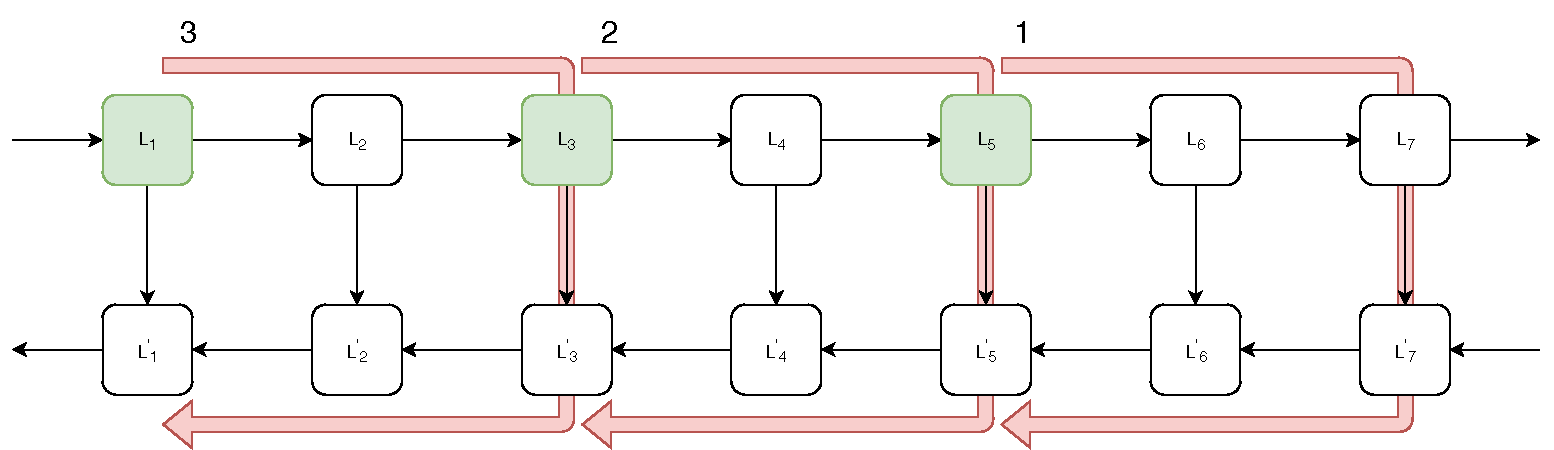
\includegraphics[width=0.92\linewidth]{backprop_segmented.pdf}
    \caption{Segmented backpropagation with checkpointing: Say we are computing the backward pass. The forward pass has already been computed, and only the outputs of \(L_1\), \(L_3\), and \(L_5\) were stored. Then, to perform the backward pass, we perform backproagation (both forward and backward) for segments 1, then 2, then 3, as shown.}
    \label{fig:1-backprop-segmented}
\end{figure}

The question now becomes of solving for the optimal checkpointing policy: which tensors to checkpoint, how many to checkpoint, and how best to exploit multiple recomputations, such as to satisfy the memory budget with the least computational cost. The solution depends on the precise memory budget and per-layer compute and memory costs. Gruslys et al. form DeepMind solve this for Recurrent Neural Networks (RNNs) using dynamic programming \cite{Gruslys2016}. However, RNNs comprise a sequence of solely the same layer repeated many times, giving uniform per-layer compute and memory costs - a very simplifying assumption that does not hold for almost all neural networks. I will rectify this limitation in this thesis.

Furthermore, popular ML frameworks like TensorFlow \cite{tensorflow2015-whitepaper}, MxNet \cite{mxnet2015}, and PyTorch \cite{Paszke2017} have very limited support for checkpointing. PyTorch, MxNet, and a third-party TensorFlow library by OpenAI \cite{Salimans2018} have similar functionality. They force the user to specify the number of segments and will split the sequence evenly, or ask the user to choose the checkpoints. They do not support multiple recomputations. TensorFlow's internal graph optimiser Grappler employs a non-optimal, user-guided, greedy, heuristic-based approach that finds the backward nodes in the computational graph, selects their inputs and the user-specified inputs as candidates for dropping, then does so until the memory budget is satisfied. Moreover, Grappler, in my opinion, requires non-trivial effort on the user's behalf to manually configure.

Clearly, the checkpointing support in these frameworks is behind research. I have chosen to improve PyTorch as it is one of the most popular frameworks, and because it lends itself nicely to extension in the manner desired \todo{elaborate}.

Specifically, to improve upon the above discussed limitations of checkpointing, I will make the following contributions in this thesis:
\begin{itemize}[topsep=0pt]
    \item Generalise the dynamic programming technique proposed by DeepMind to solve for the optimal checkpointing policy of a feedforward neural network given \textit{arbitrary} per-layer compute and memory costs and the memory budget.
    \item Provide an implementation of this technique in PyTorch that allows the user to overcome out-of-memory errors with minimal effort. Given only the user's existing sequential network, it will:
    \begin{enumerate}
        \item Profile the precise per-layer costs;
        \item Solve for the optimal checkpointing policy;
        \item Present a helper function that can be called in the user's training loop to execute the sequence according to the policy, satisfying the memory budget.
    \end{enumerate}
\end{itemize}
